\documentclass[a4paper,11pt, twocolumn]{article}
\usepackage[margin=0.8in]{geometry}
\usepackage{xcolor}
\usepackage{graphicx} %package to manage images
\graphicspath{ {./images/} }
\usepackage{float}

\title{AS-3 Timing Circuits}
\author{Revision sheet}
\date{}

\usepackage{fancyhdr}
\pagestyle{fancy}
\fancyhead{} % clear all header fields
\renewcommand{\headrulewidth}{0pt} % no line in header area
\fancyfoot{} % clear all footer fields
\renewcommand{\footrulewidth}{0.4pt}
\fancyfoot[C]{\thepage} % page number in centre of the page
\fancyfoot[R]{\footnotesize Thomas Boxall \\ Images from the WJEC E-Book} % right hand footer has author name on top line and images reference on bottom line
\fancyfoot[L]{\footnotesize AS-3 Timing Circuits \\ Revision sheet} % left hand footer has title of document on top line and 'Revision Sheet' on bottom line


\begin{document}

\maketitle
\thispagestyle{fancy}

% CONTENTS OF THE REVISION SHEET HERE
\section{Capacitors}
\begin{figure}[H]
    \centering
    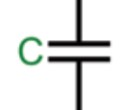
\includegraphics[width=0.2\textwidth]{images/capacitor.jpg}
    \caption{Circuit symbol for a capacitor}
    \label{fig:capacitor}
\end{figure}
\noindent Capacitors store charge. The equation\\
$\displaystyle Q=CV$ \\
can be used to calculate how much charge is stored in the capacitor. The unit of capacitance (C) is the Farad (F). Usually a capacitor will be in the region of micro/ nano/ pico farads.
\subsection{Series And Parallel}
The total capacitance of capacitors in series can be calculated using the following formula:\\
$\displaystyle \frac{1}{C_{total}} = \frac{1}{C_1} + \frac{1}{C_2} + \frac{1}{C_3}+ ...$\\
The total capacitance of capacitors in parallel can be calculated using the following formula:\\
$\displaystyle C_{total} = C_1 + C_2 + C_3 + ...$
\subsection{Time Constant}
When a resistor and capacitor are connected in series, they form a RC network. The equation $T=R\times C$ links them together, where T is the time constant and is measured in seconds.
\subsection{Charging A Capacitor}
The circuit below can be used to charge a capacitor.
\begin{figure}[H]
    \centering
    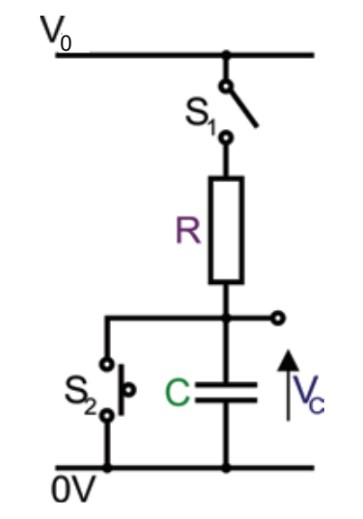
\includegraphics[width=0.3\textwidth]{images/chargingCapacitor.jpg}
    \caption{Circuit for charging a capacitor}
    \label{fig:chargingCapacitor}
\end{figure}
\noindent We'll assume that the capacitor is initially fully discharged, therefore $V_C = 0$. When we close the switch, capacitor starts charging and current `flows'. As the capacitor charges, the rate of charging slows down. A larger resistor will cause slower charging, therefore with 0 resistance, the capacitor would charge `instantly'. In the diagram above, the purpose of $\mathrm{S_2}$ is to discharge the capacitor so that the experiment can be repeated.
\begin{figure}[H]
    \centering
    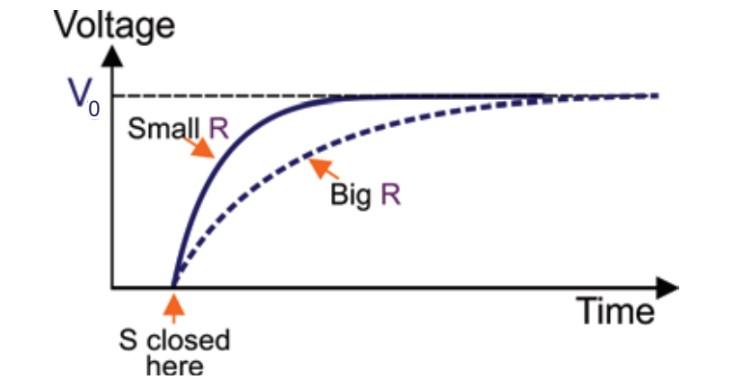
\includegraphics[width=0.4\textwidth]{images/chargingCapGraph.jpg}
    \caption{Graph showing voltage change over time when charging a capacitor}
    \label{fig:chargingCapacitorGraph}
\end{figure}
\noindent The equation to find the voltage over the capacitor ($V_C$) at a given time ($t$) is given below.\\
$ \displaystyle V_C = V_0 \left(1-e^{ \displaystyle -\frac{t}{RC}} \right)$\\
The time taken to get a certain voltage over the capacitor equation (for charging) can be seen below.\\
$\displaystyle t = -RC \ln \left(\displaystyle 1- \frac{V_C}{V_0}\right)$
\subsubsection{General Rules}
$V_C = 0.5V_0$ after $0.69RC$ ($V_C$ = half the supply voltage)\\
$V_C \approx V_0$ (fully charged) after $5RC$.

\subsection{Discharging Capacitors}
The circuit below can be used to discharge a capacitor.
\begin{figure}[H]
    \centering
    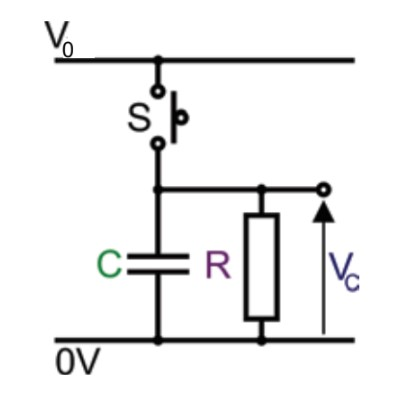
\includegraphics[width=0.3\textwidth]{images/dischargeCapacitor.jpg}
    \caption{Circuit for discharging a capacitor}
    \label{fig:dischargeCapacitor}
\end{figure}
\noindent Pressing switch $S$ instantly charges the capacitor. Discharging begins when S is released. C discharges through R.
\begin{figure}[H]
    \centering
    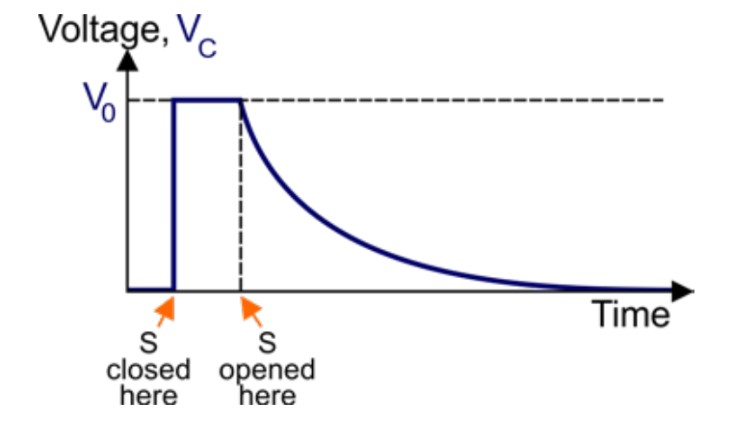
\includegraphics[width=0.4\textwidth]{images/dischargeCapGraph.jpg}
    \caption{Graph showing voltage change over time when discharging a capacitor}
    \label{fig:dischargeCapGraph}
\end{figure}
The equation to find the voltage over the capacitor ($V_C$) at a given time ($t$) is given below.\\
$\displaystyle V_C = V_0 e^{\displaystyle-\frac{t}{RC}}$\\
The time taken to get a certain voltage over the capacitor equation (for discharging) can be seen below.\\
$\displaystyle t=-RC \ln \left(\displaystyle \frac{V_C}{V_0}\right)$
\subsubsection{General Rules}
$V_C=0.5V_0$ after $0.69RC$\\
$V_C \approx 0V$ after $5RC$ (fully discharged)

\section{Monostable Circuits}
A monostable is a circuit which produces a single timing pulse. It has only one stable state; which it stays in until triggered, then it moves to the unstable state for a set period of time then returns to the stable state.
\begin{figure}[H]
    \centering
    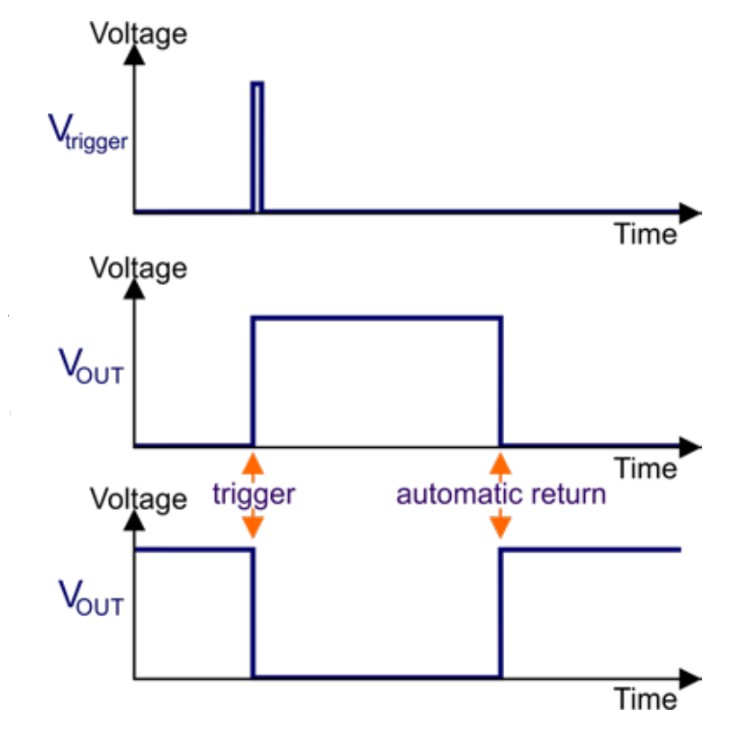
\includegraphics[width=0.4\textwidth]{images/monoBehav.jpg}
    \caption{Monostable circuit behaviour}
    \label{fig:monoBehav}
\end{figure}
\subsection{NOT Gate Monostable}
NOT gates have something called a switching threshold - this is the point at which they will invert their input. This can be used to design a NOT gate monostable.
\begin{figure}[H]
    \centering
    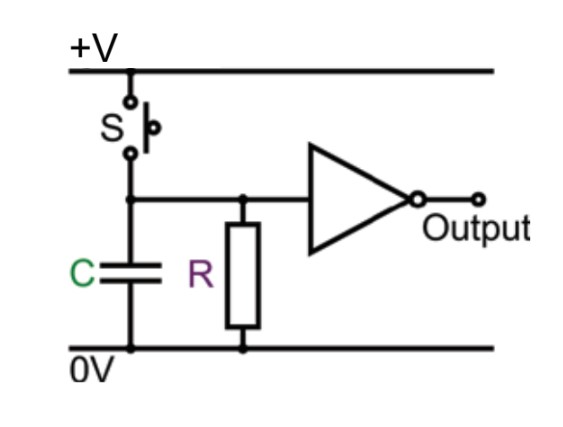
\includegraphics[width=0.3\textwidth]{images/monoNot.jpg}
    \caption{Circuit for a NOT gate monostable}
    \label{fig:monoNot}
\end{figure}
\noindent The output of the monostable can be shown on a graph.
\begin{figure}[H]
    \centering
    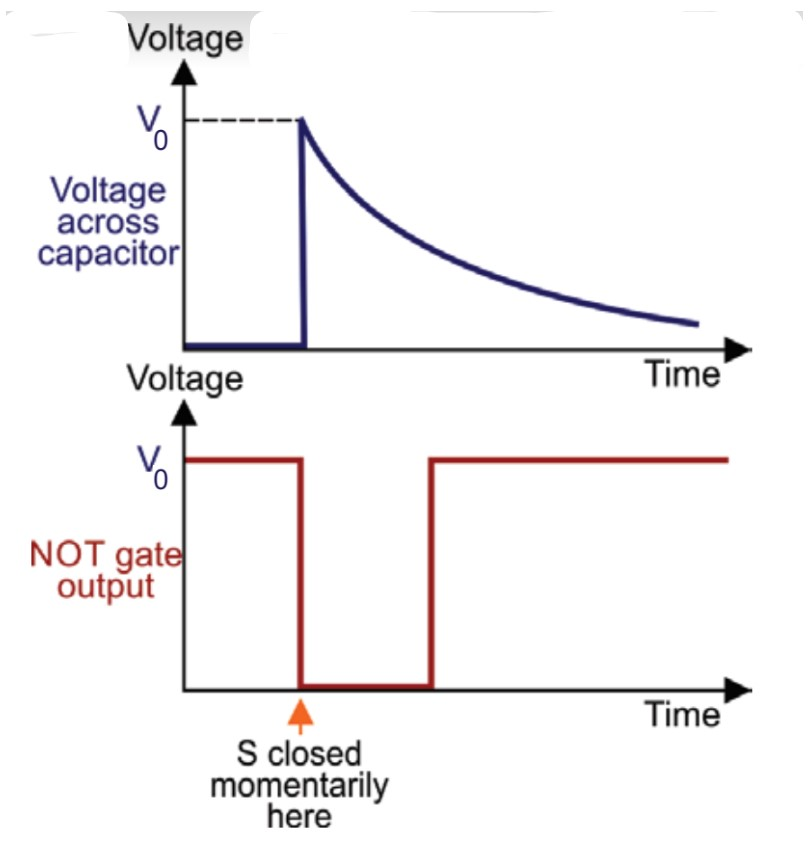
\includegraphics[width=0.4\textwidth]{images/monoNotGraph.jpg}
    \caption{Graph showing the NOT gate monostable}
    \label{fig:monoNotGraph}
\end{figure}
\subsubsection{Delayed Response Monostable}
The resistor can be moved and another switch added which gives a circuit that produces a delay before triggering the monostable.
\begin{figure}[H]
    \centering
    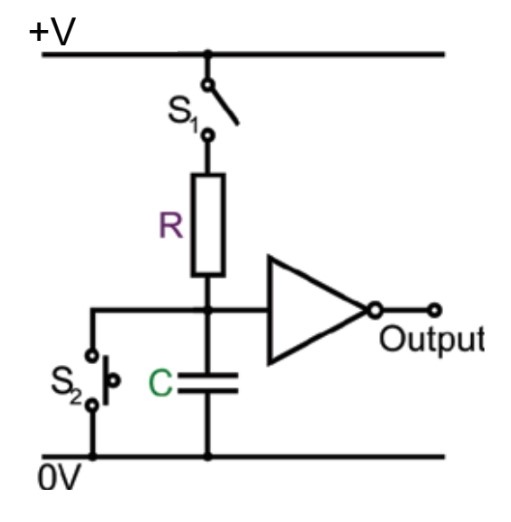
\includegraphics[width=0.3\textwidth]{images/monoNot2.jpg}
    \caption{Circuit for a delayed NOT monostable}
    \label{fig:monoNot2}
\end{figure}
\noindent This gives us the following graphed output.
\begin{figure}[H]
    \centering
    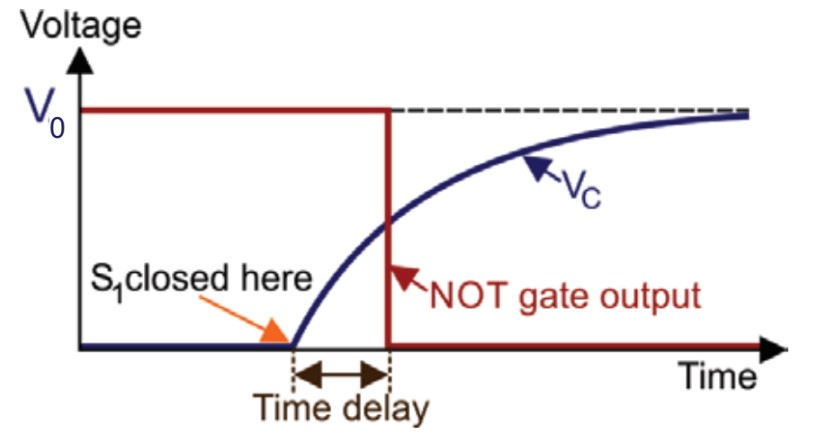
\includegraphics[width=0.4\textwidth]{images/monoNotGraph2.jpg}
    \caption{Graph showing the delayed NOT gate monostable}
    \label{fig:monoNotGraph2}
\end{figure}
\subsection{555 Timer Monostable}
The 555 Timer IC can be used to build a monostable as seen below.
\begin{figure}[H]
    \centering
    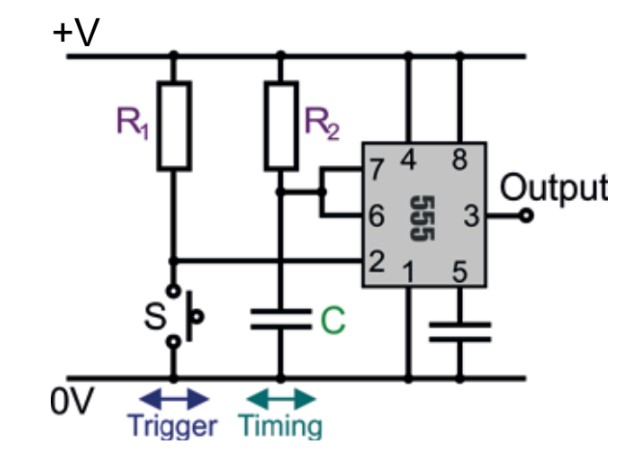
\includegraphics[width=0.3\textwidth]{images/mono555.jpg}
    \caption{Circuit for a 555 timer monostable}
    \label{fig:mono555}
\end{figure}
\noindent $T=1.1RC$ where resistor used is $R_2$.\\
Once the button is pressed, the monostable triggers and behaves as expected. You cannot re-trigger the 555 monostable mid pulse by pressing the button down again. The output will stay high all the time the button is pressed, even if T is over.
\subsection{Uses Of Monostables}
Monostables can be used to de-bounce a switch. 

\section{Astable Circuits}
These have no stable states. They oscillate between on and off. The time on ($T_H$) is called a Mark and the time off ($T_L$) is called a space. The time period can be calculated as follows:\\
$T = T_L + T_H$. The time on and time off do not have to be equal. The following graph shows this.
\begin{figure}[H]
    \centering
    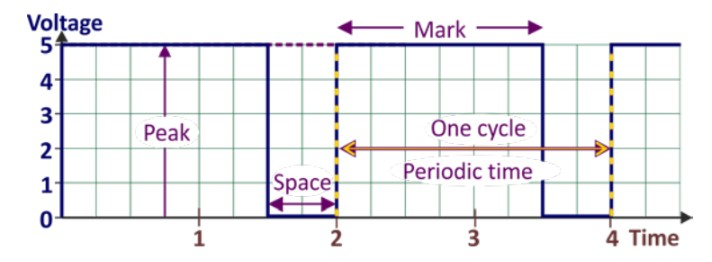
\includegraphics[width=0.4\textwidth]{images/astable.jpg}
    \caption{Graph showing the behaviour of an astable}
    \label{fig:astable}
\end{figure}
\noindent The output is a square wave. The frequency can be calculated using the equation seen below.\\
$\displaystyle f = \frac{1}{t} = \frac{1}{T_H + T_L}$
\subsection{Schmitt Inverter Astable}
A Schmitt Inverter can be used to build an astable. It has upper and lower switching thresholds which makes it really useful for this. It's upper threshold is $\frac{2}{3}V_S$ and its lower threshold is $\frac{1}{3}V_S$. The Schmitt Inverter Astable has the following circuit diagram.
\begin{figure}[H]
    \centering
    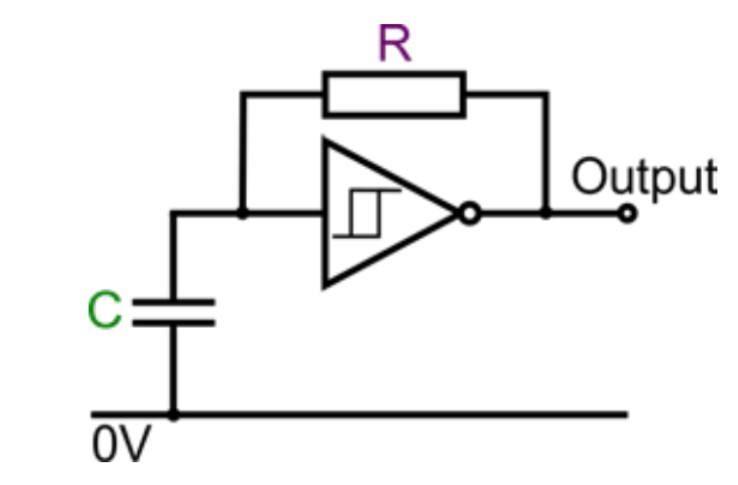
\includegraphics[width=0.3\textwidth]{images/astaSchmitt.jpg}
    \caption{Circuit for a Schmitt inverter astable}
    \label{fig:astaSchmitt}
\end{figure}
\noindent This produces the following output graph.
\begin{figure}[H]
    \centering
    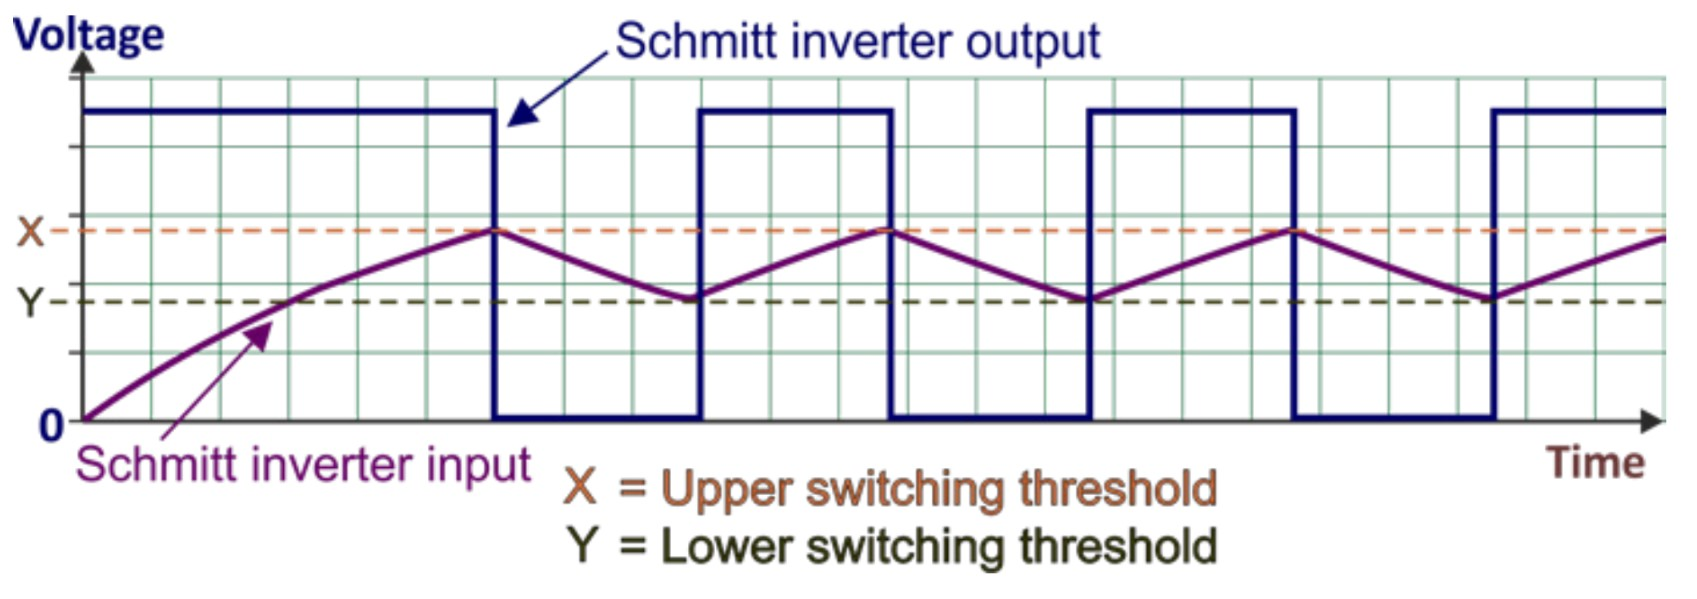
\includegraphics[width=0.4\textwidth]{images/astaSchmittGraph.jpg}
    \caption{Graph showing the inputs, output and switching thresholds of a Schmitt inverter astable}
    \label{fig:astaSchmittGraph}
\end{figure}
\noindent The Mark:Space ratio will always be 1:1 and the equation for frequency is as follows.\\
$\displaystyle f = \frac{1}{RC}$
\subsection{555 Timer Astable}
\begin{figure}[H]
    \centering
    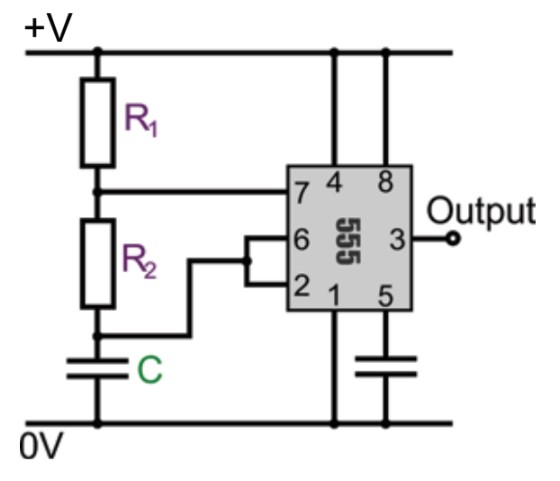
\includegraphics[width=0.3\textwidth]{images/asta555.jpg}
    \caption{Circuit for a 555 timer astable}
    \label{fig:asta555}
\end{figure}
\noindent The capacitor charges through $R_1$ and $R_2$, providing the time on\\
$\displaystyle T_H = 0.7 (R_1 + R_2) C$\\
The capacitor discharges through $R_2$, providing the time off\\
$T_L = 0.7 R_2 C$\\
The frequency can be calculated with the following equation\\
$\displaystyle f= \frac{1.44}{(R_1 + 2R_2)C}$\\
The Mark-Space ratio can be calculated using one of the following equations, to one.\\
$\displaystyle \frac{T_H}{T_L} = \frac{R_1 + R_2}{R_2} = \frac{T_{on}}{T_{off}} : 1$\\
It is impossible to have a Mark-Space ratio of 1:1, however if $R_2 >> R_1$, $\displaystyle \frac{T_H}{T_L}$ can be closer to 1.



\end{document}
